\documentclass[tikz,border=1pt]{standalone}
\usetikzlibrary{calc}
\usepackage{tikz}
\usetikzlibrary{arrows}

\usepackage{color}
\pagecolor{white}

\begin{document}

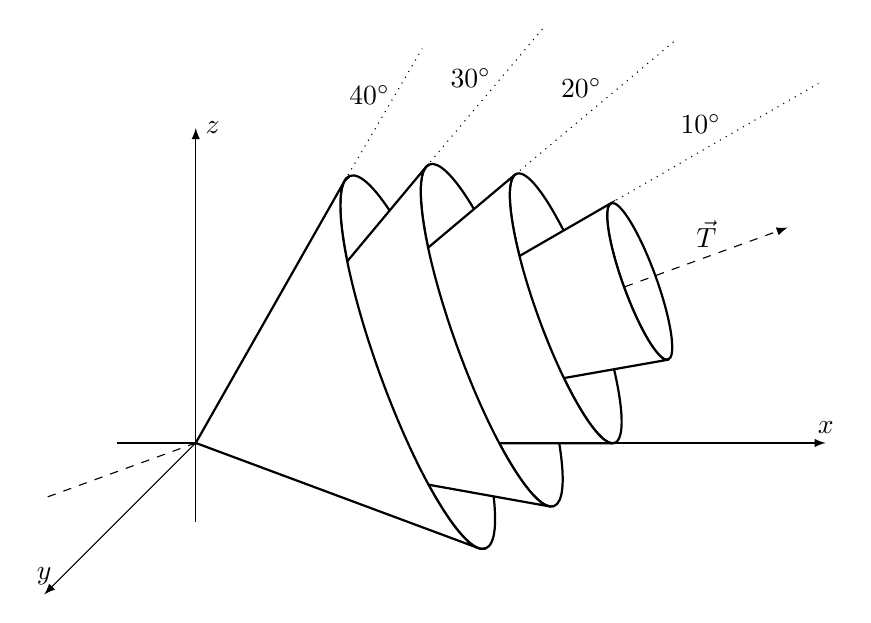
\begin{tikzpicture}[scale=1,rotate=20]

\draw[-latex,rotate=-20] (xyz cs:x=-1) -- (xyz cs:x=8) node[above] {$x$};
\draw[-latex,rotate=-20] (xyz cs:y=-1) -- (xyz cs:y=4) node[right] {$z$};
\draw[-latex,rotate=-20] (xyz cs:z=-1) -- (xyz cs:z=5) node[above] {$y$};

\foreach \x in {4,...,1}  
\draw[black,thick] ({7-\x},{tan(\x*10)*(7-\x)}) arc (90:360+90:{tan(\x*10)*(7-\x)*0.2} and {tan(\x*10)*(7-\x)});

\foreach \x in {1,...,4}  
{
\filldraw[black,thick,fill=white] ({(7-\x)-0.2*0.2*tan(\x*10)*(7-\x)*tan(\x*10)*(7-\x)/(7-\x)},{-tan(\x*10)*(7-\x)*sqrt(1-0.2*0.2*tan(\x*10)*(7-\x)/(7-\x)*tan(\x*10)*(7-\x)/(7-\x))}) -- (0,0) -- ({(7-\x)-0.2*0.2*tan(\x*10)*(7-\x)*tan(\x*10)*(7-\x)/(7-\x)},{tan(\x*10)*(7-\x)*sqrt(1-0.2*0.2*tan(\x*10)*(7-\x)/(7-\x)*tan(\x*10)*(7-\x)/(7-\x))}) -- ({(7-\x)},{tan(\x*10)*(7-\x)}) arc (90:270:{tan(\x*10)*(7-\x)*0.2} and {tan(\x*10)*(7-\x)});
	
}

\foreach \x in {1,...,4}  
{
\draw[dotted] ({(7-\x)-0.2*0.2*tan(\x*10)*(7-\x)*tan(\x*10)*(7-\x)/(7-\x)},{tan(\x*10)*(7-\x)*sqrt(1-0.2*0.2*tan(\x*10)*(7-\x)/(7-\x)*tan(\x*10)*(7-\x)/(7-\x))}) -- ({1.5*(7-\x)-0.2*0.2*tan(\x*10)*(7-\x)*tan(\x*10)*(7-\x)/(7-\x)},{1.5*tan(\x*10)*(7-\x)*sqrt(1-0.2*0.2*tan(\x*10)*(7-\x)/(7-\x)*tan(\x*10)*(7-\x)/(7-\x))})	node[pos=0.5,above] {$\x0^\circ~~~$};
}

%\foreach \x in {1,...,4}  
%{
%\filldraw[black,fill=white]
%(0,0) --  ({-(7-\x)+0.2*0.2*tan(\x*10)*(7-\x)*tan(\x*10)*(7-\x)/(7-\x)},{tan(\x*10)*(7-\x)*sqrt(1-0.2*0.2*tan(\x*10)*(7-\x)/(7-\x)*tan(\x*10)*(7-\x)/(7-\x))}) -- ({-(7-\x)},{tan(\x*10)*(7-\x)}) arc (90:270:{tan(\x*10)*(7-\x)*0.2} and {tan(\x*10)*(7-\x)}) -- (0,0);
%	
%}

\draw[-latex,dashed] (5.8,0) -- (8,0) node[pos=0.5,above] {$\vec{T}$};
\draw[dashed] (-2,0) -- (0,0);
%\draw[latex-] (-7.5,0) -- (-6.2,0) node[pos=0.5,below] {$\mathbf{T}'$};

\end{tikzpicture}

\end{document}